% latex template for a report
% written by Michael McClintock

\RequirePackage[l2tabu, orthodox]{nag} % warnings for obsolete stuff
\documentclass[12pt,a4paper]{article}  % article class

% font setup
\usepackage{ifluatex}
\ifluatex
    \usepackage[no-math]{fontspec} % keep standard math
    \setmainfont[Ligatures=TeX]{Linux Libertine}
    \setsansfont[Ligatures=TeX]{Linux Biolinum}
    \setmonofont[Ligatures=TeX]{Inconsolata}
\else
    \usepackage[T1]{fontenc}
    \usepackage{inconsolata}
\fi
\usepackage{microtype}

% useful packages
\usepackage[svgnames]{xcolor}          % color commands
\usepackage{graphicx}                  % including graphics (use eps)
\usepackage[margin=20mm]{geometry}     % set margins
\usepackage{amsmath,amssymb,cancel,bm} % math \bm for bold math
\usepackage[hidelinks]{hyperref}       % clickable links
\usepackage{url}                       % format urls
\usepackage{cleveref}                  % convenient refrencing use \Cref
\usepackage{paralist}                  % compact itemize/enumerate
\usepackage[hang, small, bf, margin=20pt]{caption} % captions for figures
\usepackage{setspace}\onehalfspacing               % 1.5 line spacing
\setlength{\parindent}{0cm}\usepackage{parskip}    % paragraph skip
\usepackage[                                   % SI units
    load-configurations=abbreviations,         % unit abrev.
    separate-uncertainty=true,                 % plus minus in uncertainty
    inter-unit-product=\ensuremath{{}\cdot{}}, % dot between units
    per-mode=symbol-or-fraction                % per style
]{siunitx}
\usepackage[nottoc,numbib]{tocbibind} % refs in toc

\begin{document}

% title page
\begin{titlepage}
\begin{center}
\textsc{\LARGE PHYS3900 Final Project}\\[1cm]
{\LARGE Smartphone Based Physics Learning}\\[2cm]
\begin{minipage}[t]{0.6\columnwidth} \large
\begin{description}
\itemsep2mm
\small
\item [\emph{Author:}] Michael McClintock (41757129)
\item [\emph{Partner:}] Alex van Nunen
\item [\emph{Date:}] October 8, 2012
\item [\emph{Email:}] michael.mcclintock@uqconnect.edu.au
\item [\emph{Supervisors:}] Dr. Tim McIntyre, Dr Margaret Wegener
\end{description}
\end{minipage}
\vfill
\end{center}
\end{titlepage}

% abstract
\begin{abstract}
Ab.
\end{abstract}
\thispagestyle{empty}
\newpage

% table of contents
\tableofcontents
\thispagestyle{empty}
\newpage
\setcounter{page}{1}

% sections
\section{Introduction and Background}

% It is no secret that smartphones, tablets and other portable
% multimedia devices are on the rise. As reported in February 2012,
% 487.7 million smartphones were shipped worldwide 2011.  This figure,
% up 63\% from 2010, also meant that smarthphone sales have overtaken
% the sale of personal computers \cite{canalys}. 

% There are a number of factors that make smartphone based learning
% (often referred to as ubiquitous learning or just ``u-learning") an
% effective, if not inevitable, complement to the more traditional
% methods of course and content delivery. These factors include the
% widespread smartphone reliance of university students and staff, high
% convenience, powerful multimedia capabilities and good wireless and
% internet connectivity \cite{worry}.

% While many universities have developed campus-wide tools for
% smartphones. The use of u-learning solutions tailor-made for specific
% courses or subject areas is not widely accepted \cite{procsmart}.
% One reason is the lack of mature technology for content delivery that
% addresses technical issues such as platform independence. Another is the
% lack of examples and trials related to the design of content for
% u-learning systems.

% This project has two separate goals. The first is to find a simple
% solution that allows the delivery of u-learning content to smartphones
% and tablets. The second and more important goal is to produce and test
% some u-learning material for first year physics students.

% While subject specific u-learning material is a relatively new concept
% there is a great deal of research into what makes good ``e-learning"
% material where e-learning refers to the use of computers and internet
% in learning. Many of the generally accepted approaches to e-learning
% may be equally effective when transferred to a smartphone based
% system.

% \section*{Significance of Research and Expected Outcomes}

% Any method or aid that helps students absorb and understand a topic at
% a fundamental level is valuable to instructors. Finding this type of
% tool for physics is even more significant because the ideas and
% concepts of physics are generally more abstract and fundamental
% compared to other subject areas. 

% Designing, implementing and testing a u-learning system for a small
% part of a first year physics course allows for evaluation of the
% effectiveness of smartphone based systems. Following this project
% instructors should have some evidence of the advantages or
% disadvantages of u-learning systems for first year physics. As well as
% some ideas about how to create their own systems.

\section{Methodology and Design}

The conventional method for creating mobile applications (apps) is called native app development and the process depends heavily on the mobile operating system. The advantages of the "native" approach is that apps are very responsive (fast) and have full access to device specific features. On the other hand creating native apps takes time, significant platform specific knowledge and programming skills.

A number of different mobile operating systems have emerged each with their own specific ecosystem of tools for creating native apps. For example there is iOS (Apple), Android (Google), Windows Phone (Microsoft), WebOS (HP), Blackberry OS and Bada (Samsung). The reality is that students will have smartphones with a variety of different operating systems.

For this project we decided to take a "web" based approach for creating the mobile applications (apps). The main reason for this choice was platform independence. Every mobile operating system has a web browser that when given some HTML input will render more or less the same output across all devices and operating systems.

Below is an outline of the process we used.
\begin{enumerate}
\item Create the content.
\item Convert the content into HTML and include additional libraries that make the result look and feel like a native app.
\item For each platform (iOS, Android, etc..) make a simple native "wrapper" that runs a web browser to view the result.
\end{enumerate}
The following sections will describe each step in more detail.

\subsection{Creating the content}

The target audience for the apps were first year science students studying PHYS1171 at the University of Queensland. PHYS1171 is an introductory physics course with a focus on biological applications. We focused on writing content for the fluid part of the course. This included topics such as pressure, Pascal's Principle, buoyancy, non-viscous flow and viscous flow.

\subsubsection{Content format}

Before writing the content we needed to choose a format. We asked ourselves, what is an effective way to author content for a physics app? Below are some characteristics of the content format which we thought were important.

\begin{itemize}
\item First the format should be simple. The generation of quality physics content is what the author should be focusing on. The format shouldn't get in the way. It should be simple enough that anyone can write content for the apps.
\item The format should be a well established standard with tested tools for conversion to other formats.
\item It should be easy to insert text, math equations, images, videos links and references.
\item A plain text, freely available solution is desirable.
\end{itemize}

Using the above characteristics the format we decided to use for this project was Markdown \cite{md}. Perhaps the best way to describe Markdown is by example. \Cref{fig:md} shows some markdown text along with the final output on a mobile device. The example shows a heading, an image, text and a math equation (using tex notation).

\begin{figure}[htb]
\rule[0.5ex]{1\columnwidth}{1pt}
\footnotesize
\begin{verbatim}
# Buoyancy

![ ](/static/Fluid3.png)

Take the block of water inside the bucket on the left hand side. This
block of water is being upheld by the pressure in the liquid
underneath the block of water, while being pressed down by the force
of gravity.  Since this block of water is stationary, that means that
the force of gravity equals the force of buoyancy. So at this point:

$F_{gravity}=F_{buoyant}=m_f g$
\end{verbatim}
\rule[0.5ex]{1\columnwidth}{1pt}
\\[2mm]
\centering
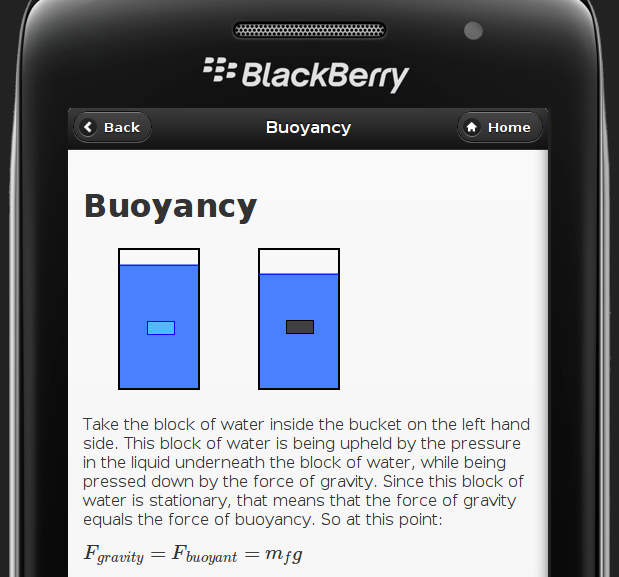
\includegraphics[width=0.45\textwidth]{buoyancy.png}
\caption{Markdown input (top), Final output (bottom)}
\label{fig:md}
\end{figure}

\subsubsection{Content Structure}

The idea of the physics app is to give students access to extra content that reinforces concepts taught in lectures and in textbooks. It was our goal to produce small modules which could be read in approximately 5 minutes. These modules generally included some images and text and were written in an informal, friendly style.

The following directory structure was used (.md is the extension of a markdown file)
\begin{itemize}
\item content (folder containing all the content)
\begin{itemize}
\item classes (folder containing all the classes)
\begin{itemize}
\item classes.md (short description of the app)
\item PHYS1171 (folder containing PHYS1171 specific content)
\begin{itemize}
\item PHYS1171.md (short description of PHYS1171)
\item buoyancy.md
\item pressure.md
\item pascal.md
\item viscous.md
\item nonviscous.md
\end{itemize}
\end{itemize}
\end{itemize}
\item static (all images go in this folder)
\end{itemize}

This directory structure was designed to be simple and generic. It is remarkably easy to add new modules and even classes to the app. For example to add a new class just create a new folder in the classes directory and add some content. When the app is generated all the navigation menus will be updated and the new content added.

\subsubsection{Collaboration and Version Control}

In order to collaborate with other content authors and to manage different versions. The whole project was managed using Git \cite{git} and hosted online at Github \cite{github}. While these tools are usually associated with software development they work extremely well for any text based projects and provide a well established environment for collaboration. 

\subsection{Transforming the content into a "Web App"}

The previous section detailed the method we used to generate content. The next task was to take all the content and transform it into a "web app". A "web app" is basically a whole bunch of web files (Usually HTML, Javascript, CSS, Images). When these files are loaded into a browser you get the look and feel of a mobile phone application. 

The main idea that we used when generating the app is that the resulting web app is a function of the the following input
\begin{itemize}
\item The content (markdown files)
\item The static content (mainly images)
\item Javascript files (3rd party libraries for buttons, math rendering, etc.)
\item Style files (CSS files for things like font sizes and colours)
\item HTML templates (provide the framework of the app where content gets inserted)
\end{itemize}

By using an automated system we were able to effectively "compile" the web app. In other words we could write content and hit compile and the web app was ready to be packaged and distributed.

\subsection{Packaging and Distributing the App}

The last part of the process is to package the "web app" and provide a means for users to install the app. We used an online build service called PhoneGap Build \cite{phonegap} to automate this. PhoneGap Build takes a directory of web files (web app) and creates packaged native applications for a wide array of mobile operating systems including iOS and Android. When the packaged application is executed the web files are loaded into the device browser. So the result looks and feels like a standard app (see \Cref{fig:md}).

Finally PhoneGap Build provides a website where users can download and test the packages (shown in \Cref{fig:pg}). At this stage after thorough testing the apps could be submitted to the respective App Stores for each platform and could be installed by anyone.

\begin{figure}[htb]
\centering
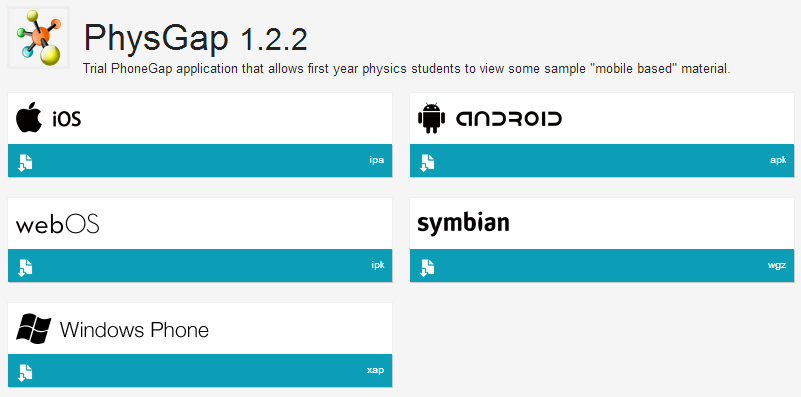
\includegraphics[width=0.9\textwidth]{phonegap.png}
\caption{PhoneGap Build website for the packaged apps.}
\label{fig:pg}
\end{figure}

\subsection{Receiving feedback from students}

In order to receive feedback on the App and the physics content, we created an online survey where students can answer questions and leave comments. We were very interested in how students used the app. Below are some questions from the survey

\begin{itemize}
\item What type of device was used?
\item Did the app work? If not what was the issue?
\item Was the app helpful?
\item Did the app help in understanding the lecture topics?
\item Was the format pleasing?
\item What was the best thing about the app?
\item What could be improved?
\item Would you use this app?
\end{itemize}

The results will be discussed in the following section.

\section{Results}

We were able to build apps for 5 different platforms (iOS, Android, webOS, Symbian and Windows Phone) of which we were able to test the final product on both iOS and Android. By following the methodology described above we succeeded in producing apps for multiple platforms created from the same content source. After supplying the content it takes about 3 minutes to update and rebuild the apps for all 5 platforms.

We authored 5 modules for students to read (See \Cref{fig:menu}) complete with images, equations and accompanying text. All the code and content for this project is available at:
\begin{quote}\url{https://github.com/mmcclintock/physgap}\end{quote}
The apps are available at:
\begin{quote}\url{https://build.phonegap.com/apps/195010/share}\end{quote}

\begin{figure}[htb]
\centering
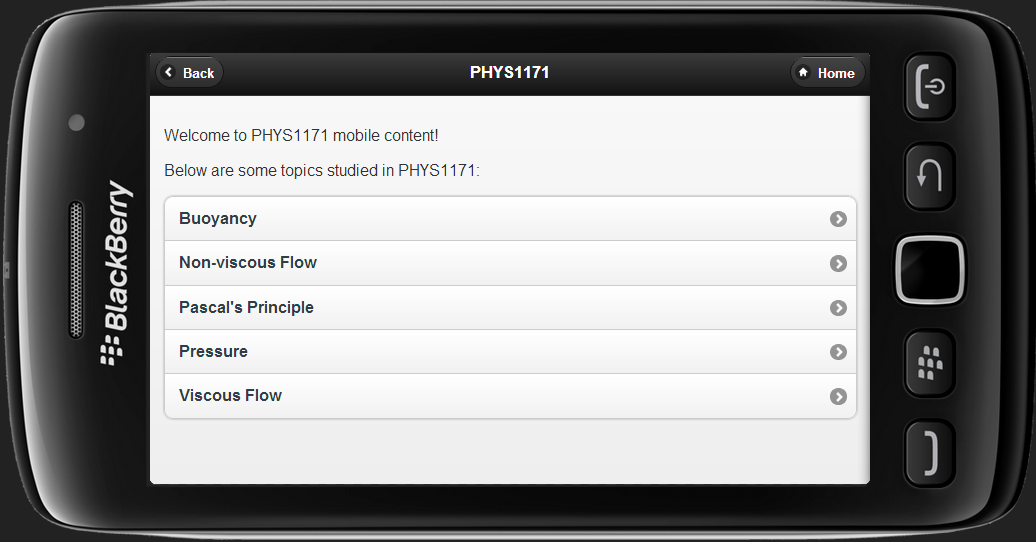
\includegraphics[width=0.9\textwidth]{menu.png}
\caption{Shows a menu for the 5 modules we created for the app.}
\label{fig:menu}
\end{figure}

\subsection{Student Feedback}

In the short time we were allocated for this project we decided to focus on building a working mobile application with sample content that students may actually find useful. As a result we did not have time or the means to launch large-scale testing where we could objectively analyze the quality and effectiveness of the app. However we did receive some feedback from students some of which we will discuss in this section.

23 students responded to our online survey leaving feedback for the app. The students were asked a review the app by rating various aspects on a scale from 1 to 5. 1 being the worst and 5 being the best. Here are the average ratings for some questions.

\begin{itemize}
\item Was the app helpful? 4.09
\item Was the format pleasing? 3.95
\item Would you use this app? 4.56
\item Did the app help me understand Pascal's Principle? 3.5 
\item Did the app help me understand buoyancy? 3.3
\item Did the app help me understand Bernoulli's Principle? 3.3
\item Did the app help me understand viscous flow? 3.3
\end{itemize}

While these results are promising we were more interested in hearing student comments about what they liked or didn't like about the app. Here are some student comments.

\rule[0.5ex]{1\columnwidth}{1pt}
"Loaded quickly with Google Chrome. More user interaction. A glossary of terms. More specific info to know what the questions in the Pre-reading quizzes ask."
\\[3mm]
"General writing could be improved, worked examples need more working with clear explanations beside it. Annotated pictures and deconstruction of equations would be appreciated."
\\[3mm]
"It is an app for phones, this itself is the best thing. Include in it all content taught in the course."
\\[3mm]
"The text posed questions that provoked thought...about principles. Bravo! The text then gave answers. Do more of that bite-sized stuff. Continue to speak in everyday language, where possible, while still being scientific. Keep provoking thought, dig deeper, give answers, reinforce with with visual examples of why things work the way they do."
\\[3mm]
"Easy to use, easy to access and good information. Could have questions to test understanding."
\\[3mm]
"It divided the relevant material into clearly decipherable categories and provided useful visual aid. The issue with the 'math processing errors' meant that I missed out on a great deal of potentially useful information and the examples didn't make as much sense."
\\[3mm]
"More convient and accessible. Definitely get it up and running for apple iphones as majority of people will have this and use them" \\
\rule[0.5ex]{1\columnwidth}{1pt}

\subsection{Li}


\section{Discussion}

\section{Summary}

\section{Self Assessment}

\bibliographystyle{ieeetr}
\bibliography{refs}

\end{document}